\chapter{数学分析}{
\section{映射与函数}{

\subsection{映射}{
    映射指的是集合之间的一种对应关系.

    定义 : $X,Y$是两集合,按照某个规则$f$,对于任一的$x \in X$,有唯一的$y \in Y$与之对应,则称$f$是$X$到$Y$的一个映射.

    记为 : $f: X \to Y$,即 : $x \mapsto y = \defFunction{x}$

    称呼 :

    \begin{itemize}
        \item $y$ : 在映射$f$下,x的像.
        \item $x$ : 在映射$f$下,y的\textcolor{red}{一个}逆像.
        \item $X$ : $f$的定义域,记为$X = D_f$.
        \item $Y$ : $f$的值域,记为$R_f \subset Y$,具体的来说,$R_f = \set{y | y \in Y \land \exists x(y = f(x) \land x \in X)}$
    \end{itemize}

    举例 : 设$X$是平面上三角形的全体,$Y$是平面上圆的全体,构造一个映射$f$,表示(y 是 x 的外接圆),记为 : $$
        f : \underset{x \mapsto y}{X \to Y}
    $$

    \subsubsection{映射的基本要素}{
        \begin{itemize}
            \item $X = D_f$,定义域.
            \item $Y$,限制值域的范围.
            \item $f$,需要保证像的唯一性.
        \end{itemize}

        这说明了两点 : \begin{enumerate}
            \item {
                  映射的像是唯一的,举例 :

                  设$X = \mathRealNumberCollection^+ = \set{x | x \in R \land x > 0}$,假设存在映射$f : \underset{x \mapsto y}{X \to Y}(y^2 = x)$,此时$Y = \mathRealNumberCollection$,那么假设$x = 4,y = \pm 2$.这个映射就无法保证像的唯一性.换句话说,这个$f$并不是个映射.

                  但是可以稍作改造:对$Y = \mathRealNumberCollection$做限制,令$Y = R^-$,此时 : $$
                      \mapsToWithSubText{f}{X \to Y}{x \mapsto y}(y^2 = x)
                  $$
                  就构成了一个映射
                  }
            \item {
                  映射不要求逆向唯一.
                  }
        \end{enumerate}
    }%映射的基本要素结尾

    \subsubsection{映射的分类}{
        \begin{itemize}
            \item {
                  单射 :

                  $f$是$X$到$Y$的一个映射,若逆像也具有唯一性,则称$f$是单射(injection)

                  逻辑命题表述 : $x_1 \neq x_2 \Rightarrow y_1 \neq y_2(y_1 = \defFunction{x_1},y_2 = \defFunction{x_2})$

                  注 : 单射的值域不一定完全等于$Y$,也可能包含于$Y$,即$R_f \subseteq Y$
                  }
            \item {
                  满射 : 如果映射的值域完全等于$Y$,即$R_f = Y$,则称为满射(surjection).

                  注 : 满射不一定是单射
                  }
            \item {
                  双射 : 如果$f$又是单射,又是满射,则称$f$为双射(bijection)

                  双射又称为一一对应.
                  }
        \end{itemize}
    }%映射的分类结尾

    \subsubsection{逆映射}{
        如果$f : X \to Y$是一个单射,即对任意的$y \in R_f$,有唯一的逆像$x \in X$与$y$对应.

        如果$\mapsToWithSubText{g}{R_f \to X}{y \mapsto x}$是满射($\defFunction{x} = y$)

        那么$g$就称为$f$的逆映射,又记为$f\inverse$

        举例 : $\mapsToWithSubText{y = \sin x}{\mediumBigCase{-\frac{\pi}{2},\frac{\pi}{2}} \to \mediumBigCase{-1,1}}{x \mapsto y = \sin x}$,他的逆映射为 : $$
            \mapsToWithSubText{x = \arcsin y}{\mediumBigCase{-1,1} \to \mediumBigCase{-\frac{\pi}{2},\frac{\pi}{2}}}{y \mapsto x}(\sin x = y)
        $$
    }%逆映射结尾

    \subsubsection{复合映射}{
        $$
            \mapsToWithSubText{g}{X \to U_1}{x \mapsto u = g(x)}
        $$
        $$
            \mapsToWithSubText{f}{U_2 \to Y}{u \mapsto y = f(u)}
        $$

        这两个映射若是要复合在一起,那么就得满足 : $R_g \subset U_2 = D_f$.即 : $g$的值域在$f$的定义域中,才能构造出复合映射.

        称为$f$与$g$的复合映射.

        例 : 设$X = Y = U_1 = U_2 = \mathRealNumberCollection$ :
        $$
            \mapsToWithSubText{g}{x \to U_1}{x \mapsto u = \sin x}
        $$
        $$
            \mapsToWithSubText{f}{U_2 \to Y}{u \mapsto y = \frac{u}{1 + u^2}}
        $$
        由于$R_g = \mediumBigCase{-1,1} \subset D_f$,所以 : $$
            \mapsToWithSubText{f \cdot g}{X \to Y}{x \mapsto y = \frac{\sin x}{1 + \sin x}}
        $$
    }%复合映射结尾

}%映射结尾

\subsection{函数}{
函数是映射的特殊情况.

有映射 : $$
    \mapsToWithSubText{f}{X \to Y}{x \mapsto y = \defFunction{x}}
$$
如果$X \subset \mathRealNumberCollection,Y = \mathRealNumberCollection$,即如果两者都是实数构成的集合,那么就称$f$为一元实函数(简称函数).

如果$X$是卡氏积(笛卡尔乘积集合),那么就是多元实函数.

对函数来说,映射可以简写为 : $$
    y = \defFunction{x},x \in X\ (X = D_f)
$$
其中$x$也称为自变量,$y$称为因变量,函数也反映了因变量与自变量变化的一种因果关系.

\subsubsection{基本初等函数}{
    以下几种函数被称为基本初等函数 :

    \begin{enumerate}
        \item 常数函数 : $y = \mathConstant$
        \item 幂函数 : $y = x^\alpha\ (\alpha \in \mathRealNumberCollection)$
        \item 指数函数 : $y = a^x\ (a > 0 \land a \neq 1)$
        \item 对数函数 : $y = \log_ax\ (a > 0 \land a \neq 1)$
        \item 三角函数 : $y = \sin x,\cos x,\tan x,\cot x...$
        \item 反三角函数 : $y = \arcsin x,\arccos x,\arctan x...$
    \end{enumerate}
}%基本初等函数结尾

\subsubsection{初等函数}{
    初等函数是由基本初等函数经过有限次四则运算与复合运算所产生的函数.

    例如 : $$
        y = ax^2 + bx + c
    $$
}%初等函数结尾

\subsubsection{自然定义域}{
自然定义域是指函数中自变量的最大取值范围.

如果函数不注明定义域,则默认定义域为他的自然定义域.

例 : 求$y = x + \frac{1}{x}$的自然定义域 : $$
    D = (-\infty,0) \unionSet (0,+\infty),\ R = (-\infty,-2] \unionSet [2,+\infty)
$$

方法不说了...难以描述.
}%自然定义域结尾

\subsubsection{函数的表示}{
    \begin{itemize}
        \item 显式表示 : $y = \defFunction{x}$
        \item {
              分段表示 :

              $A \intersectionSet B = \emptyset$,现有$\varphi(x)$定义于$A$上,$\psi(x)$定义于$B$上,构造函数$\defFunction{x}$ : $$
                  \defFunction{x} = \begin{cases}
                      \varphi(x)\qquad x \in A \\
                      \psi(x)\qquad x \in B
                  \end{cases}
              $$

              这样的表示称为函数的分段表示.
              }
        \item {
              隐函数表示(函数的隐式表示) : $F(x,y) = 0$

              也就是说没有写成$y = F(x)$的形式,而是写成了方程的形式,式中$y$与$x$的变化关系并没有写出,而是写在方程中.

              例如 : $$
                  x^2 + y^2 = R^2\mbox{或者}x^2 + y^2 - R^2 = 0
              $$

              发现对任意的$x \in (-\mathRealNumberCollection,+\mathRealNumberCollection)$,都有两个$y$与之对应.

              这并不意味着这个函数关系无法讨论,只需要对$y$做限制,比如要求$y \geq 0$,这样一来对于给定的$y$,就有唯一确定的$x$,由此就构成了函数关系.

              需要注意的是并不是所有的隐函数都可以写出显式表达的形式,比如Kepler方程 : $$
                  y = x + \varepsilon \sin y
              $$

              这个方程描述了行星绕太阳运行的轨迹的规律,轨迹是个椭圆.其中$\varepsilon$是这个椭圆的离心,$x$与时间有关,$y$与行星的位置有关.
              }
        \item {
              参数表示 :

              当$x$与$y$的关系不方便表示的时候可以考虑引进参数$t$($t$只是个字符),如果$x$和$y$可以表示成$t$的函数 : $$
                  \begin{cases}
                      x = x(t) \\
                      y = y(t)
                  \end{cases},\ t \in [a,b]
              $$

              这样就间接的反映了变量$y$与$x$之间的参数表示,称为函数的参数表示.

              他是这么表示的 : 有两个集合 : $$
                  X = \set{x | x = x(t),t \in [a,b]},\ Y = \set{y | y = y(t),t \in [a,b]}
              $$

              那么函数关系$f$就是一个映射 : $$
                  \mapsToWithSubText{f}{X \to Y}{x = x(t) \mapsto y = y(t)}
              $$
              }
    \end{itemize}
}%函数的表示结尾

\subsubsection{函数的简单性质}{
    \begin{enumerate}
        \item {
              有界性 : 对于$y = \defFunction{x},x \in D$ :

              如果存在$m < M$,使得$m \leq \defFunction{x} \leq M,x \in D$,则称$\defFunction{x}$有界,$m$称为下界,$M$称为上界.

              等价定义 : 存在$X > 0$(此$X$不是集合),使得$\absoluteValue{\defFunction{x}} \leq X,x \in D$

              需要注意的是 : 如果函数有界,那么上下界是不唯一的.
              }
        \item {
              单调性 : 对于$y = \defFunction{x},x \in D$ :

              若对于任意的$x_1,x_2 \in D,x_1 < x_2 \Leftrightarrow \defFunction{x_1} \leq \defFunction{x_2}$,则称函数$f$在$D$单调增加.如果$\leq$可以换成$<$,则称为严格单调增加.

              记为 : $$
                  f\uparrow(f\mbox{严格}\uparrow)
              $$

              类似的,将不等号的箭头方向改变,也有单调减少和严格单调减少,记为 : $$
                  f\downarrow(f\mbox{严格}\downarrow)
              $$
              }
        \item {
              奇偶性 : 设函数的定义域$D$关于原点对称.即 : $$
                  x \in D \Leftrightarrow -x \in D
              $$
              那么 :

              \begin{itemize}
                  \item 若在$D$上,$f(x) = f(-x)$,则称$f$是偶函数.
                  \item 若在$D$上,$f(x) = -f(x)$,则称$f$是奇函数.
              \end{itemize}
              }
        \item {
              周期性 : 设$D$是函数$f$的定义域,$x \pm T \in D$,并且$f(x) = f(x \pm T)$

              $T$称为函数的一个周期.

              在所有的周期中,如果有最小的$T$,则称他为最小周期.

              }
    \end{enumerate}
}%函数的简单性质结尾

\subsubsection{一些特殊的函数}{
    \begin{itemize}
        \item {
              符号函数 :

              符号函数(Sign function,简称sgn)是一个逻辑函数,用以判断实数的正负号.为避免和英文读音相似的正弦函数(sine)混淆,它亦称为Signum function.其定义为 : $$
                  sgn(x) = \begin{cases}
                      -1\qquad x < 0 \\
                      0\qquad x = 0  \\
                      1\qquad x > 0
                  \end{cases}
              $$

              \functionTabular{$D = (-\infty,+\infty)$}{$R = sgn(x) = \set{-1,0,1}$}{奇函数}

              图像为 :

              \begin{center}
                  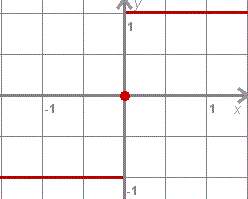
\includegraphics[scale=0.5]{resources/Signum_function.png}
              \end{center}
              }
        \item {
              整数部分函数(下取整函数) :$$
                  y = [x]
              $$

              在数学和计算机科学中,取整函数是一类将实数映射到相近的整数的函数.

              常用的取整函数有两个,分别是下取整函数和上取整函数.

              下取整函数即为取底符号,在数学中一般记作$[x]$或者$E(x)$,在计算机科学中一般记作$floor(x)$,表示不超过$x$的整数中最大的一个 : $$
                  [x] = \min\set{n \in \mathIntegerCollection | x \leq n}
              $$

              \functionTabular{$D = (-\infty,+\infty)$}{$R = [X] = \mathIntegerCollection$}{N/A}

              图像为 :

              \begin{center}
                  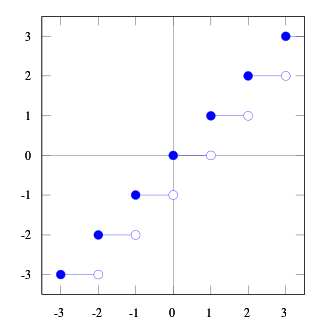
\includegraphics[scale=0.5]{resources/Floor_function.png}
              \end{center}

              下取整函数的符号用方括号$[x]$表示,称作高斯符号.
              }
        \item {
              小数部分函数(分数部分函数) : $$
                  y = (x) = x - [x]
              $$

              小数部分函数(decimal part function)亦称分数部分函数,是一种特殊的数论函数.$x$的小数部分记为${x}$,读作$x$的小数部分(或分数部分).小数部分函数被定义为${x}=x-[x]$,其中$[x]$是整数函数.$\{x\}$只能是0或正的纯小数,即$\{x\}$满足$0≤\{x\}<1$

              \functionTabular{$D = (-\infty,+\infty)$}{$R = \{X\} = (0,1)$}{N/A}

              图像为 :

              \begin{center}
                  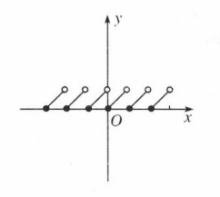
\includegraphics[]{resources/DecimalPartFunction.png}
              \end{center}
              }
        \item {
              狄利克雷函数 :

              问 : 是否周期函数都有最小周期?

              答 : 不是.

              反例 : 狄利克雷函数(Dirichlet function)$D(x)$ : $$
                  D(x)
                  =
                  \begin{cases}
                      0\qquad \mbox{$x$无理数} \\
                      1\qquad \mbox{$x$有理数}
                  \end{cases}
              $$

              \functionTabular{$D = (-\infty,+\infty)$}{$R = D(x) = (0,1)$}{偶函数}

              任何的有理数$r > 0$都是他的周期,没有最小周期.
              }
    \end{itemize}
}%一些特殊的函数结尾

}%函数结尾

}%映射与函数结尾

\section{数列极限}{

\subsection{实数系的连续性}{

\subsubsection{引入}{
    一切都得从实数系的诞生说起 :

    命题 : $\sqrt{2}$不是有理数.

    \begin{center}
        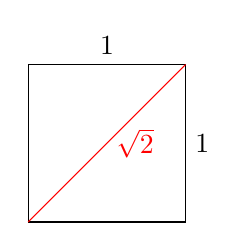
\begin{tikzpicture}
            \draw (0,0) -- (0,2) --node[above]{$1$} (2,2) -- node[right]{$1$} (2,0) -- cycle;
            \draw[red] (0,0) --node[right]{$\sqrt{2}$} (2,2);
        \end{tikzpicture}
    \end{center}

    使用反证法

    如果$\sqrt{2}$不是有理数,设其为有理数,即 : $$
        \sqrt{2} = \cfrac{n}{m}
    $$

    其中$n,m \in \mathNatureNumberCollection^+$且互质.

    那么$2 = \cfrac{n^2}{m^2}$,即$n^2 = 2m^2$

    则$n$是偶数.令$n = 2k$,则$m^2 = 2k^2$,因此$m$也是偶数,矛盾,得证.

    \qed

    换句话来说,在有理数上开根号不封闭,因此需要扩展数系.

    从几何上看是这样的 :

    \begin{center}
        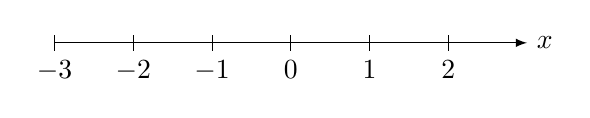
\begin{tikzpicture}% table%\begin{}[]%\addplot table[] {};%\end{}%\end{}
            \draw[-latex] (0,0) -- (6,0) node[right]{$x$};
            \foreach \i in {-3,...,2}{
                    \draw (\i + 3,-0.1) node[below]{$\i$} -- (\i + 3,0.1);
                }
        \end{tikzpicture}
    \end{center}

    \begin{itemize}
        \item {
              $\mathIntegerCollection$ :

              整数集上每一个数都对应其上的一个点,每两个点之间总有距离,点与点之间距离至少为1.称这一性质为\textcolor{red}{离散性}.

              因此可以说 : 整数集合具有集散性.
              }
        \item {
              $\mathRationalNumberCollection$ :

              有理数集合种每一个元素都可以在数轴上找到一个点与他对应,而且有理数很多,多到无法找到一个小区间,使得这个小区间内没有有理数.将这种性质称为\textcolor{red}{稠密性}.

              因此可以说 : 有理数集合具有稠密性.
              }
        \item {
              $\mathRealNumberCollection$

              长期以来人们一直只认识有理数,直到公元200年前的古希腊 :

              \begin{center}
                  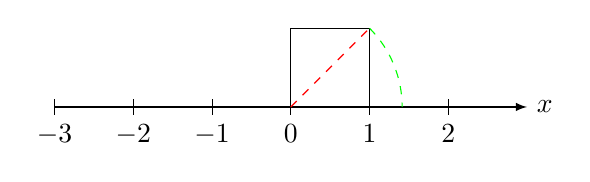
\begin{tikzpicture}
                      \draw[-latex] (0,0) -- (6,0) node[right]{$x$};
                      \foreach \i in {-3,...,2}{
                              \draw (\i + 3,-0.1) node[below]{$\i$} -- (\i + 3,0.1);
                          }
                      \draw (3,0) rectangle (4,1);
                      \draw[dashed,red] (3,0) -- (4,1);
                      \draw[dashed,green] (4,1) arc (45:0:{sqrt(2)});
                  \end{tikzpicture}
              \end{center}

              就这样,人们发现了一个在数轴上的点,对应的不是有理数.

              换句话说,尽管有理数集合在数轴上有稠密性,但是有空隙.

              于是又扩展了数系,将无限不循环小数(即无理数)加进了有理数系,就这样出现了实数集合$\mathRealNumberCollection$,自此运算又封闭了.

              因此实数是有理数集合和有理数集合的并,即 : $$
                  \mathRealNumberCollection = \set{x | x \in \mathRationalNumberCollection \lor x\mbox{是无理数}}
              $$

              引入的无理数填满了数轴上的空隙,现在数轴上每一个点都与实数集合中的一个元素对应,换句话来说: 实数集合布满了整个数轴,不留任何空隙.称这一性质为\textcolor{red}{连续性}.

              即 : 实数的连续性.

              实数集合有时候又被称为实数连续统.
              }
    \end{itemize}
}%引入结尾

\subsubsection{最大数与最小数}{
    首先提出以下概念 : 最大数与最小数.

    $S \subset \mathRealNumberCollection,\ S \neq \emptyset$,如果$S$是有限集,则$S$必有最大数和最小数.

    但是如果$S$是无限集,则$S$不一定有最大数与最小数.

    \begin{itemize}
        \item 如果$\exists \xi \in S$,使得$\forall x \in S$,有$x \leq \xi$,则称$\xi$是$S$中的最大数,记为$\xi = \max S$
        \item 如果$\exists \eta \in S$,使得$\forall x \in S$,有$x \geq \eta$,则称$\eta$是$S$中的最小数,记为$\eta = \min S$
        \item 显然,有限数集合一定有最大数和最小数.
        \item 但是无限数集合则不一定.
    \end{itemize}
}%最大数与最小数结尾

\subsubsection{上确界与下确界}{
    \begin{itemize}
        \item {
              上界 :

              \begin{itemize}
                  \item 设$S \subset \mathRealNumberCollection,\ S \neq \emptyset$,如果$\exists M \in \mathRealNumberCollection$,使得$\forall x \in S$,有$x \leq M$,则称$M$是$S$的一个上界,或称$S$有上界.
                  \item 设$U$是$S$上界的集合,则$U$没有最大数,但$U$必定有最小数.
                  \item $U$中的最小数记为$\beta = sup S$,称为$S$的上确界(supremum).
                  \item {
                        \(
                        \beta : \begin{cases}
                            \beta\mbox{是上界,即 : }\forall x \in S(x \leq \beta) \\
                            \beta\mbox{是最小上界,即 : }\forall \epsilon > 0 \exists x \in S (x > \beta - \epsilon)
                        \end{cases}
                        \)
                        }
              \end{itemize}
              }
        \item {
              下界 :

              \begin{itemize}
                  \item 设$S \subset \mathRealNumberCollection,\ S \neq \emptyset$,如果$\exists m \in \mathRealNumberCollection$,使得$\forall x \in S$,有$x \geq m$,则称$m$是$S$的一个下界,或称$S$有上界.
                  \item 设$L$是$S$下界的集合,则$L$没有最小数,但$L$必定有最大数.
                  \item $L$中的最大数记为$\alpha = inf S$,称为$S$的下确界(infimum).
                  \item {
                        \(
                        \alpha : \begin{cases}
                            \alpha\mbox{是下界,即 : }\forall x \in S(x \geq \alpha) \\
                            \alpha\mbox{是最大下界,即 : }\forall \epsilon > 0 \exists x \in S (x < \alpha + \epsilon)
                        \end{cases}
                        \)
                        }
              \end{itemize}
              }
    \end{itemize}
}%上确界与下确界结尾

\subsubsection{确界存在定理(实数系连续性定理)}{
\begin{itemize}
    \item 非空有上界的数集必有上确界.
    \item 非空有下界的子集必有下确界.
\end{itemize}

证明 : $$
    \forall_{x \in \mathRealNumberCollection} (x = [x] + (x))
$$

$$
    (x) = 0.a_1 a_2 \dots a_n \dots
$$
说明 :
\begin{itemize}
    \item 将$(x)$写成无限小数表示
    \item 如果是有限小数,那么后面加一列0.
    \item $0.a_1a_2 \dots a_p 000\dots\ (a_p \neq 0)$可以写成$0.a_1a_2 \dots (a_p-1)999\dots$,这两者等价$(1 = 0.99999\dots)$,但是一般使用前者的形式表示
\end{itemize}

设$S \subset \mathRealNumberCollection,S \neq \emptyset,$有上界,$S$可以表示成为 : $$
    S = \set{a_0 + a_1a_2 \dots a_n \dots | a_0 = [x],0.a_1a_2 \dots a_n \dots = (x),x \in S}
$$
\begin{enumerate}
    \item $S$有上界,取$S$中所有$a_0$的最大值,记为$\alpha_0$
    \item 作$S_0 = \set{x | x \in S \land [x] = \alpha_0}$,则$x \in S \land x \notin S \Rightarrow x < \alpha_0$
    \item 取$S_0$中$x$的小数表示中第1位小数的最大者为$\alpha_1$.
    \item 作$S_1 = \set{x | x \in S_1 \land x\mbox{的第一位小数为}\alpha_1}$,则$x \in S \land x \notin S_1 \Rightarrow x < \alpha_0 + 0.\alpha_1$
    \item 一般的,取$S_{n - 1}$中$x$的小数表示中第$n$位的最大者为$\alpha_n$
    \item 那么$S_n = \set{x | x \in S_{n - 1} \land x\mbox{的小数第$n$位为}\alpha_n}$,则$x \in S \land x \notin S_n \Rightarrow x < \alpha_0 + 0.\alpha_1\alpha_2 \dots \alpha_n \dots$
    \item \begin{enumerate}
              \item 得到了一串集合$S \supset S_0 \supset S_1 \supset S_2 \supset \dots \supset S_N \supset \dots$
              \item $\alpha_0 \in \mathIntegerCollection,\alpha_n(\alpha_1,\alpha_2,\dots,\alpha_n,\dots) \in \set{0,1,2,\dots,9}$
          \end{enumerate}
    \item 令$\beta = a_0 + 0.\alpha_1\alpha_2 \dots \alpha_n \dots$
    \item {
          \begin{proof}
              $\beta$是$S$的上确界 :

              \begin{enumerate}
                  \item $\beta$是$S$的上界 : \begin{enumerate}
                            \item $\forall x \in S$,或者$\exists n_0(x \notin S_{n_0})$,或者$\forall_{n \in \mathNatureNumberCollection}(x \in S_n)$
                            \item 若为前一种情况,则$x < \alpha_0 + 0.\alpha_1\alpha_2 \dots \alpha_n \leq \beta$
                            \item 若为后一种情况,则考虑$[x]$与$(x)$的每一位小数.发现$x = \beta$
                            \item 因此$\beta$是$S$的上界.
                        \end{enumerate}
                  \item $\beta$是最小上界,换句话来说 : $\forall \epsilon > 0,\beta - \epsilon$不是上界. : \begin{enumerate}
                            \item 可取$n_0 \in \mathIntegerCollection$,使$\cfrac{1}{10^{n_0}} < \epsilon$
                            \item 取$x \in S_{n_0}$,$[x] = \alpha_0$,前$n_0$位小数为$\alpha_1,\alpha_2,\alpha_{n_0}$
                            \item $\beta - x \leq \cfrac{1}{10^{n_0}} < \epsilon \Rightarrow x > \beta - \epsilon$
                            \item 因此$\beta$是$S$的上确界.下确界同理.
                        \end{enumerate}
              \end{enumerate}
          \end{proof}
          }
\end{enumerate}

此定理反映了实数系的连续性 :

假设数轴上存在一点为空隙,这一点既不是有理数也不是无理数,那么这个空隙左边的实数没有上确界,右边的实数没有下确界.

因此被称为实数系连续性存在定理.

$$
    \cfrac{n^2}{m^2} + \cfrac{2nr}{m} + r^2 - 2 = \cfrac{2n}{m} + r^2 - t < 0
$$
}%确界存在定理结尾

\subsubsection{Dedekind切割定理}{
    \begin{itemize}
        \item 事实上实数连续性有多种等价的叙述方式,其中之一就是从有理数集的稠密性出发,使用Dedekind切割定理.
        \item 此定理是以有理数集$Q$的切割为基础导出无理数定义,进而定义整个实数系的.
    \end{itemize}

    \begin{itemize}
        \item {
              定义1 : 设两个非空有理数集合$A$和$B$满足以下条件 : $Q$ = $A \unionSet B$.且对任意的$a \in A$与$b \in B$,成立$a < b$,则称$A$和$B$构成$Q$的一个切割,记为$A/B$.

              从逻辑上讲,对有理数集合$Q$的任何切割$A/B$,下述情况有且仅有一种出现 : \begin{enumerate}
                  \item 集合$A$有最大数$a_0$,集合$B$没有最小数.
                  \item 集合$A$没有最大数,集合$B$有最小数$b_0$
                  \item 集合$A$没有最大数,集合$B$没有最小数.
                  \item 集合$A$有最大数,集合$B$有最小数.
              \end{enumerate}

              但情况$4$是不可能发生的.因为根据切割的定理,可知$a_0 < b_0$.而$\cfrac{a_0 + b_0}{2}$显然也是$Q$中的有理数,由$a_0 < \cfrac{a_0 +b_0}{2} < b_0$,即得到$\cfrac{a_0 + b_0}{2}$既不属于$A$也不属于$B$,这就与$Q = A \unionSet B$产生矛盾.

              对于情况$1$,称切割$A/B$确定了有理数$a_0$,对于情况$2$,称切割$A/B$确定了有理数$b_0$,而对情况$3$,由于$A/B$没有确定任何有理数,即$A$与$B$之间存在一个空隙,因此有必要引进一个新的数(即无理数)作为这一切割的确定对象,并且构成了实数集$\mathRealNumberCollection$.

              引入了后就可以保证对实数集的任意切割都不会出现空隙了.
              }
    \end{itemize}

    \paragraph{Dedekind切割定理的证明}{
        Dedekind切割定理 : 设$\hat{A} / \hat{B}$是$\mathRealNumberCollection$的一个切割,$\hat{A},\hat{B}$在这里意思是非空,则或者$\hat{A}$有最大数,或者$\hat{B}$有最小数.

        \begin{proof}
            设$A$是$\hat{A}$中所有有理数所构成的集合,$B$是$\hat{B}$中所有有理数构成的集合,则$A/B$是有理数集合$Q$的一个切割.由前面所述,对于切割$A/B$,下述三种情况有且仅有一种出现 :
            \begin{enumerate}
                \item 集合$A$有最大数$a_0$,集合$B$没有最小数.
                \item 集合$A$没有最大数,集合$B$有最小数$b_0$
                \item 集合$A$没有最大数,集合$B$没有最小数.
            \end{enumerate}

            对情况1,可以证明此时$a_0$是集合$\hat{a}$的最大数,而集合$\hat{B}$没有最小数 :

            用反证法.若有$\hat{a} \in \hat{A}$,成立$a_0 < \hat{a}$,则由有理数的稠密性,在区间$(a_0,\hat{a})$中必存在有理数$a_0$.由$a < \hat{a}$,可知$a \in A$,但$a > a_0$,与$a_0$就是$A$的最大数矛盾,说明$a_0$就是集合$\hat{A}$的最大数.

            对于任意的$\hat{b} \in \hat{B}$,因为$a_0 < \hat{b}$,于是在区间$(a_0,\hat{b})$中必存在有理数$b$.由$a_0 < b$,可知$b \in \hat{B}$,但是$b < \hat{b}$,这说明$\hat{B}$没有最小数.

            对于情况2,可类似证明此时$b_0$也是集合$\hat{b}$的最小数,而集合$\hat{A}$没有最大数.

            对于情况3,切割$A/B$确定一个无理数,将该无理数记为$c$,则对任意$a \in A$与任意$b \in B$,成立$a < c < b$.

            因为无理数$c \in \mathRealNumberCollection = \hat{A} \unionSet \hat{B}$,所以只有两种可能 : 或者$c \in \hat{A}$,或者$c \in \hat{B}$.若$c \in \hat{A}$,则$c$必是$\hat{A}$的最大数.若不是则存在$\hat{a} \in \hat{A}$,成立$c < \hat{A}$,在区间$(c,\hat{a})$中取有理数$a$,由$a < \hat{a}$,可知$a \in A$,但由$c < a$,又可知$a \in B$,这就产生矛盾.

            同理.若$c \in \hat{B}$,则$c$必是$\hat{B}$的最小数.

            综合情况$123$,可知Dedekind定理成立.

        \end{proof}
    }%Dedekind切割定理的证明结尾

}%Dedekind切割定理

}%实数系的连续性

\subsection{数列极限}{

    注:本章内容可用于级数.

    注:数列不是级数,级数需要求和数列不用.

    \subsubsection{数列}{
        若函数$f$的定义域为全体正整数集合$\mathNatureNumberCollection^n$,则称
        $$
            f : \mathNatureNumberCollection^+ \to \mathRealNumberCollection,\defFunction{n} \ (n \in \mathNatureNumberCollection^+)
        $$

        为数列.因正整数集$\mathNatureNumberCollection^+$的元素可按由小到大的顺序排列,所以数列$\defFunction{n}$也可以写作 :
        $$
            a_1,a_2,a_3,\dots,a_n,\dots,
        $$

        或者可以简记为${a_n}$,其中$a_n$称为该数列的通项.

        以下为一些例子 : \begin{itemize}
            \item $\set{\cfrac{1}{x}} : \cfrac{1}{1},\cfrac{1}{2},\cfrac{1}{3},\dots,\cfrac{1}{n},\dots$
            \item $\set{\cfrac{n}{n + 3}} : \cfrac{1}{4},\cfrac{2}{5},\cfrac{3}{6},\dots,\cfrac{n}{n + 3},\dots$
            \item $\set{n^2} : 1,4,9,\dots,n^2,\dots$
            \item $\set{(-1)^n} : -1,1,-1,1,\dots,(-1)^n,\dots$
        \end{itemize}

        简而言之,所谓数列就是按照正整数编号的一串数

        注意 : 与集合不同,数列允许重复,而且有顺序.
    }%数列结尾

    \subsubsection{邻域}{
        $a$点的$\epsilon$邻域$O(a,\epsilon) = (a - \epsilon, a + \epsilon)$,用集合的写法可表示为 : $$
            \set{x | x - \epsilon < x < x + \epsilon}
        $$
    }%邻域结尾

    \subsubsection{数列极限的定义}{
        设数列${x_n}$,存在$x_0$,若对于任意给定的$\epsilon > 0$,可以找到正整数$N$,使得当$n > N$时,有 : $$
            \absoluteValue{x_n - a} < \epsilon (\mbox{或者等价的说,} x \in O(a,\epsilon))
        $$

        则称数列${x_n}$收敛于$a,a$称为数列$x_n$的极限,记作
        $$
            \limNormal{n \to \infty}x_n = a
        $$

        若不存在$a$,即数列${x_n}$没有极限,则称${x_n}$不收敛,或者称${x_n}$发散.

        \begin{itemize}
            \item 此定义等价于 : 任给$\epsilon > 0$,若在$O(a,\epsilon)$之外数列${x_n}$中的项至多只有有限个,则称数列${x_n}$收敛域极限$a$.
            \item 由此定义可知,一个数列收敛的话,收敛于那个数,这与数列的前有限项无关,因此数列改动有限项不影响数列的收敛性和极限.
            \item {
                  $\cfrac{1}{n} : 1,\cfrac{1}{2},\dots$此数列以$0$为极限

                  以零为极限的变量(此处的变量是数列)通常称为\textcolor{red}{无穷小量}.

                  $$
                      \limNormal{n \to \infty}x_n = a \Rightarrow \set{x_n - a}\mbox{是无穷小量}
                  $$
                  }
        \end{itemize}
    }%数列极限的定义结尾

    \subsubsection{一些例题}{
        \begin{enumerate}
            \item {
                  用定义证明$\set{\cfrac{n}{n + 3}}$的极限为1.

                  \begin{proof}
                      对任意给定的$\epsilon > 0$ : $$
                          \absoluteValue{\cfrac{n}{n + 3} - 1} = \cfrac{3}{n + 3} < \epsilon \Leftrightarrow n > \cfrac{3}{\epsilon} - 3
                      $$

                      取$N = \mediumBigCase{\cfrac{3}{\epsilon}} + 1$,当$n > N$时,必定满足$$
                          \absoluteValue{\cfrac{n}{n + 3} - 1} < \epsilon
                      $$因此成立.

                  \end{proof}
                  }
            \item {
                  \begin{itemize}
                      \item $\set{n^2} : 1,4,9,16,\dots$
                      \item $\set{(-1)^n} : -1,1,-1,1,\dots$
                  \end{itemize}

                  根据定义,以上数列都是发散的.
                  }
            \item {
                  $0 < \absoluteValue{q} < 1$,证明$\set{q^n}$是无穷小量.

                  \begin{proof}
                      对任意的$\epsilon > 0$ : $$
                          \absoluteValue{q^n - 0} = \absoluteValue{q^n} < \epsilon
                      $$
                      $$
                          \Leftrightarrow n\lg\absoluteValue{q} < \lg\epsilon \Leftrightarrow n > \cfrac{\lg \epsilon}{\lg\absoluteValue{q}}
                      $$

                      于是$N$只要取任意大于这玩意的正整数即可,取$N = max\bigCase{\mediumBigCase{\cfrac{\lg \epsilon}{\lg \absoluteValue{q}}},1}$当$n > N$时,$\absoluteValue{q^n - 0} = \absoluteValue{q^n} < \epsilon$

                  \end{proof}

                  注 : 根据对数列极限的定义的讨论,$N$取的太大没啥意义,可以只考虑绝对值很小的$\epsilon > 0$,不妨考虑任意给定的$0 < \epsilon < \absoluteValue{q}$.则$N$可取为$\mediumBigCase{\cfrac{\lg \epsilon}{\lg \absoluteValue{q}}}$,即$\mediumBigCase{\log_{\absoluteValue{q}}\epsilon}$,当$n > N$时,成立$\absoluteValue{q^n - 0} < \epsilon$
                  }
        \end{enumerate}

        根据数列极限的定义来证明某一数列收敛,其关键是对任意给定的$\epsilon > 0$寻找正整数$N$.在上面的立体中,$N$都是通过解不等式$\absoluteValue{x_n - a} < \epsilon$来得出的.但在大多数情况下,这个不等式并不容易解.实际上,数列极限的定义并不要求取到最好的$N$,所以在证明中常常对$\absoluteValue{x_n - a}$适度的做一些放大处理,这是种常用的技巧.以下是一些例子,描述了怎么使用这个技巧 :
        \begin{enumerate}
            \item {
                  证明$\limNormal{n \to \infty}\sqrt[n]{a} = 1,\ (a > 1)$

                  % #TODO p10
                  }
        \end{enumerate}
    }%一些例题结尾

    \subsubsection{O'Stolz(stolz)定理}{
        设$(a_n)(n > 1)$和$(b_n)(n > 1)$为两个实数数列.若$b_n$为从某项开始严格单调的无界正数数列,且有穷极限
        $$
            \limNormal{n \to \infty}\cfrac{a_{n + 1} - a_n}{b_{n + 1} - b_n} = L
        $$

        存在,则 :
        $$
            \limNormal{n \to \infty}\cfrac{a_n}{b_n} = L
        $$

        其中$L$可以为有限实数或正/负无穷.

        该定理虽然主要被用于处理数列不定型极限,但该定理在没有$\limNormal{n \to \infty}a_n = \infty$这一条件时也是成立的.虽然该定理通常是以分布$b_n$为正数数列的情形加以叙述的,但注意到该定理对分子$a_n$的正负没有限制,所以原则上把对数列$b_n$的限制条件按替换为"严格单调递减且趋于负无穷大"也是没问题的.

        与洛必达的迭代用法类似,在尝试使用此定理考察数列极限时,如果发现两个数列差分的商任然是不定型,那么可以继续用.

        注意 : 与洛必达类似,判定条件不存在不能认定极限本身不存在.
    }%O'Stolz(stolz)定理结尾

}%数列极限结尾

}%数列极限结尾

}%数学分析结尾